% Author biographies for IEEE Transactions on Computers.
% Each biography must be 145 words or less. Photos are in photos/.

\begin{IEEEbiography}[{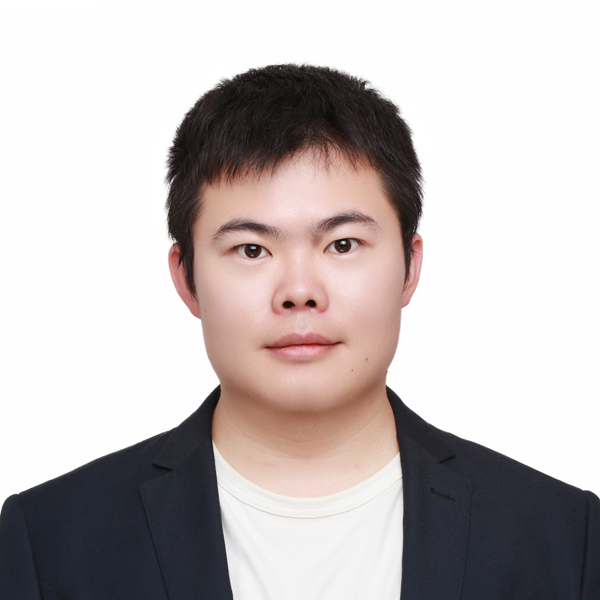
\includegraphics[width=1in,height=1.25in,clip,keepaspectratio]{photos/kexin_chu.jpeg}}]{Kexin Chu}
Kexin Chu received the B.S. and M.S. degrees in computer science
from Hefei University of Technology, Hefei, China, in 2017 and 2020,
respectively. He is currently working toward the Ph.D. degree in
computer science with the School of Computing, University of
Connecticut, Storrs, CT, USA. His research interests include machine
learning systems, large language model serving and infrastructure,
KV-cache and memory-system optimization, and trustworthy AI
infrastructure. Before beginning his doctoral studies, he was a backend
software engineer at Baidu, where he designed and maintained
large-scale production services, and he interned on model deployment
and inference optimization. His recent work focuses on efficient and
reliable LLM inference under realistic device-memory constraints,
including online precision residency for Mixture-of-Experts models.
Contact him at kexin.chu@uconn.edu.
\end{IEEEbiography}

\begin{IEEEbiography}[{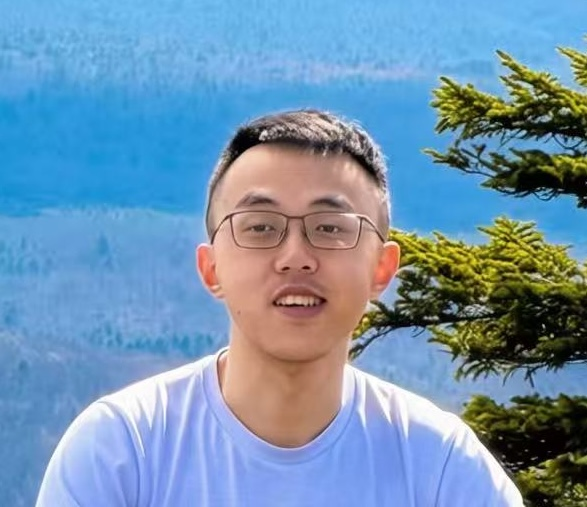
\includegraphics[width=1in,height=1.25in,clip,keepaspectratio]{photos/dawei_xiang.jpg}}]{Dawei Xiang}
Dawei Xiang received the M.S. degree in computer science and
engineering from Texas A\&M University, College Station, TX, USA, in
2024. He is currently working toward the Ph.D. degree in computer
science with the School of Computing, University of Connecticut,
Storrs, CT, USA, where he is also a research assistant. His research
interests include machine learning systems, large language model
inference, agentic workflows, and model optimization under
deployment constraints. He has worked on efficient serving and
runtime mechanisms for modern language models, with an emphasis
on Mixture-of-Experts execution when the full expert pool cannot
remain in high precision on a single GPU. Contact him at
ieb24002@uconn.edu.
\end{IEEEbiography}

\begin{IEEEbiography}[{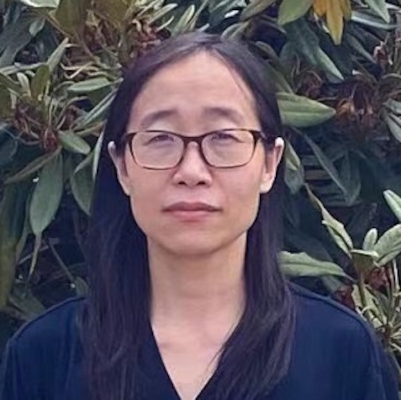
\includegraphics[width=1in,height=1.25in,clip,keepaspectratio]{photos/wei_zhang.jpg}}]{Wei Zhang}
Wei Zhang received the Ph.D. degree in computer architecture from
Beihang University, Beijing, China, in 2015, and the Ph.D. degree in
computer science from The George Washington University,
Washington, DC, USA, in 2018. She is an Assistant Professor with the
School of Computing, University of Connecticut, Storrs, CT, USA. Her
research interests include cloud computing and virtualization,
distributed systems, operating systems, resource disaggregation,
networked and storage systems, serverless computing, and machine
learning systems. Contact her at wei.13.zhang@uconn.edu.
\end{IEEEbiography}
